\chapter{Testiranje}
%\section{Opis testiranja}
Jedini pravi način da se objektivno usporedi efektivnost oba alata jest da ih se testira na realnim i konkretnim situacijama. Za testiranje će se koristiti Burp Suite Web Security Academy laboratorijske vježbe.\cite{burp_labs}
Osim što postoje vodiči za Burp Suite postoje i vodiči za ZAP koje su korisnici pisali.\cite{owasp_2fa_manual,owasp_b-f_manual}
Vježbe su odabrane uz pomoć OWASP Top 10 stranice\cite{owasp_top10} koja vodi brigu o broju i vrsti sigurnosnih rizika koji su do godine pisanja bili najčešći, 
te njihove povezane CWE-ove.
Obraditi će se laboratorijske vježbe povezane sa sigurnosnim rizicima s vrha gore navedenog popisa. Specifično su izabrane one za koje postoje rješenja u ZAP vodiču ili čija se rješenja mogu lako pronaći.
%%%%%%%%%%%%%%%%%%%%%%%%%%%%%%%%%%%%%%%%%%%%%%%%%%%%%%%%%%%%%%%%%%%%%%%%%%%%%%%%%%%%%%%%
%     SQL
%%%%%%%%%%%%%%%%%%%%%%%%%%%%%%%%%%%%%%%%%%%%%%%%%%%%%%%%%%%%%%%%%%%%%%%%%%%%%%%%%%%%%%%%
\section{Vidljiva pogreška bazirana na SQL injekciji}
%\subsection{Općenito}
SQL injekcije su među najčešćim prijetnjama na Internetu. Činjenica koje to dokazuje je da su s ostalim vrstama injekcija 2017.\ predstavljale najrasprostranjeniji sigurnosni rizik ,a 2021.\ su bile čak 
na trećem mjestu po učestalosti.\cite{owasp_top10}
SQL injekcija je tehnika napada u kojoj napadač ubacuje zlonamjerni SQL kod u polja za unos aplikacije kako bi izvršio neovlaštene radnje na bazi podataka. To 
može uključivati dobivanje osjetljivih podataka, izmjenu podataka, brisanje podataka ili izvođenje administrativnih operacija. 
SQL injekcija nastaje zbog neadekvatnog filtriranja ili validacije korisničkog unosa.\cite{clarke_sql,sql_w3}

Laboratorijska vježba sadrži ranjivost na SQL injekcije koju će biti iskorištena. Od ostalih informacija znamo da aplikacija koristi 'kolačiće' za analitiku te provodi SQL upit 
s informacijama u podnesenim kolačićima. Rezultati SQL se ne vraćaju direktno već je potrebno izazvati grešku u ispisu. Baza podataka sadrži tablicu zvanu \textit{users} sa stupcima \textit{username} i \textit{password}.
Cilj laboratorijske vježbe je pronalazak načina da web aplikaciji 'iscuri' lozinka za korisnika \textit{administrator} te se onda treba ulogirati s njihovim računom.

Ono što je također bitno za primjetiti je da se ne koriste podatci dobivene direktno iz malicioznog SQL upita, već grešku koja se zbog upita vraća. To uvelike otežava alatima da primjete takve ranjivosti kako \textit{de facto} nema polja koje bi mogli iskoristiti da nam aplikacija da neke djelove baze podataka direktno. 
Umjesto toga cilj je iskoristiti lošu obradu grešaka.\cite{sql_lab} 

\subsection{Vježba 1: Burp Suite}
Nakon otvaranja alata potrebno je kliknuti na karticu \textit{Target} kako je prikazano na slici \ref{slk:target_burp}.
\begin{figure}[H]
    \centering
    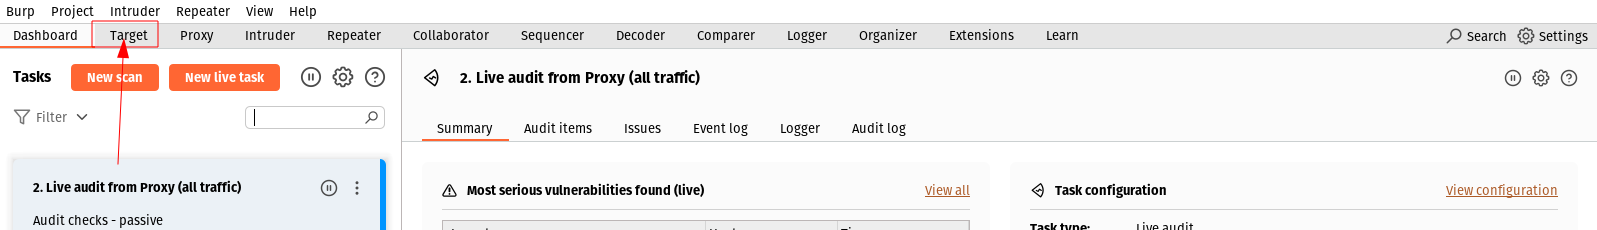
\includegraphics[width=1\textwidth]{slike/BURP_target.png}
    \caption{Popis svih kartica s naznačenom karticom \textit{Target}}
    \label{slk:target_burp}
\end{figure}

Ondje je prije svega potrebno uključiti proxy koji će biti korišten za presretanje zahtjeva i odgovora. Zatim je potrebno kliknuti na gumb \textit{Open browser} te u adresnu traku zalijepiti adresu laboratorijske
vježbe. Odmah prilikom otvaranja dediciranog pretraživača i unosom poveznice na vježbu Burp izgradi \textit{sitemap} (mapu cijele stranice).
Sada kako bi bilo moguće pronaći ranjivost koja će se iskoristiti za navedenu vježbu nužno je započeti skeniranje s kartice \textit{Dashboard > New scan > Webapp scan}.
Najprije se prikazuje pregled skena kao što je vidljivo na slici \ref{slk:burp_pojed}. Ovdje se mogu vidjeti generalne informacije o meti i trenutnim postavkama skena.
Potom se konfigurira sken kao što je to vidljivo na slici \ref{slk:burp_config}. Prilikom ove i budućih vježbi koristiti će se \textit{Deep} sken.
\begin{figure}[H]
    \centering
    \begin{minipage}[b]{0.46\textwidth}
      \centering
      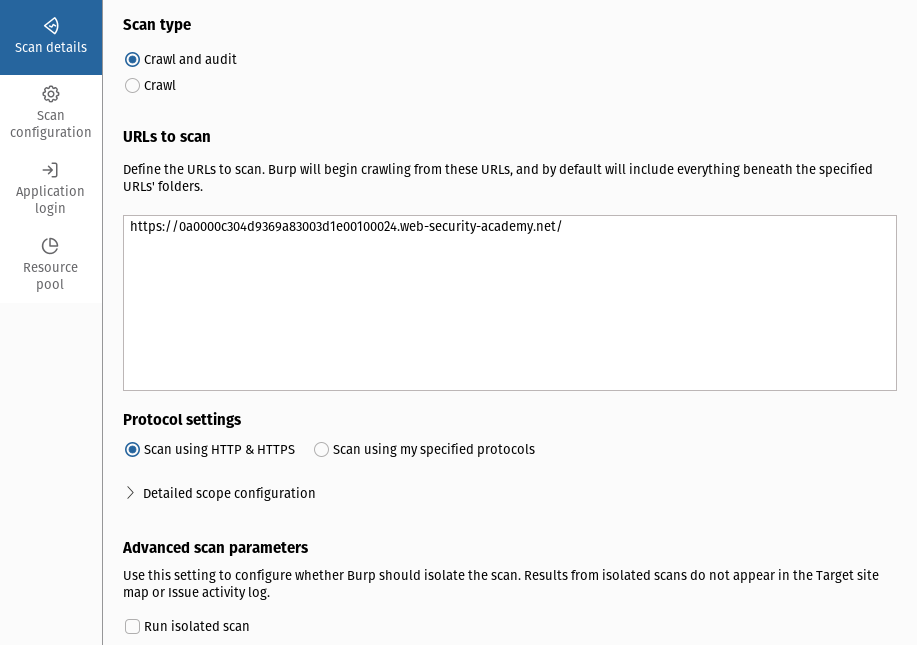
\includegraphics[width=\textwidth]{slike/scan_det.png}
      \caption{Pojedinosti skena}
      \label{slk:burp_pojed}
    \end{minipage}
    \hspace{0.05\textwidth} % Razmak između slika
    \begin{minipage}[b]{0.47\textwidth}
      \centering
      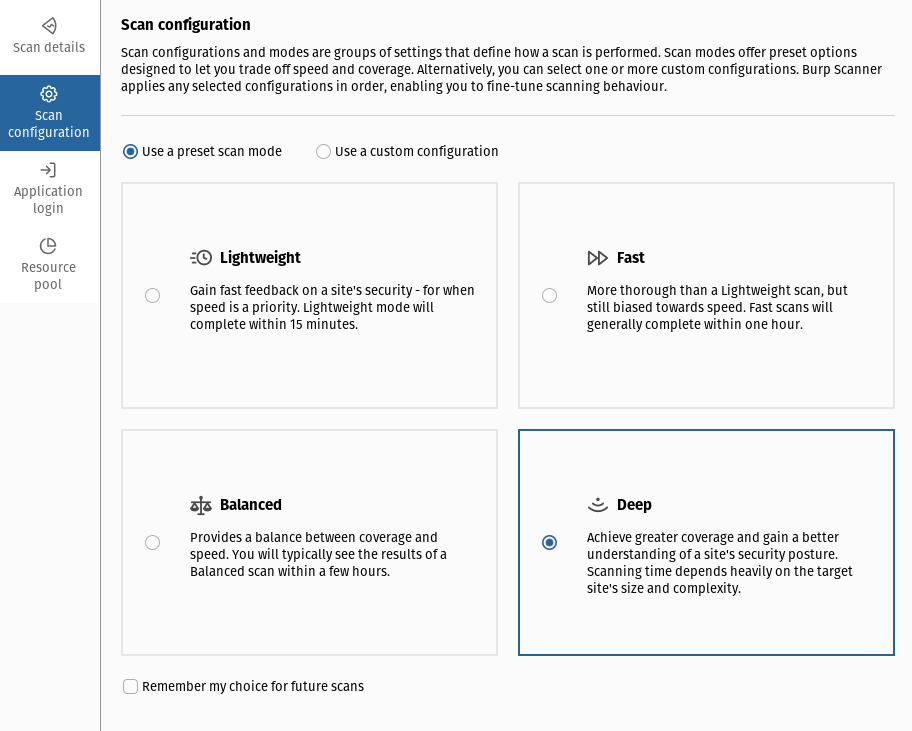
\includegraphics[width=\textwidth]{slike/scan_config_burp.png}
      \caption{Konfiguriranje skena}
      \label{slk:burp_config}
    \end{minipage}
  \end{figure}

\lstset{language=SQL}
Skeniranje traje <5 minuta te izvodi očekivane rezultate. Osim SQL ranjivosti, alat je pronašao nekolicinu informativnih detalja što se stranice tiče poput činjenice da komunikacija nije enkriptirana 
te kako nije definirana striktna sigurnosna politika za transport.
Vezano za SQL injection alat je pronašao ranjivosti na čak 3 putanje \textit{/product, /filter} i \textit{/my-account}. Za product i filter je koristio \textit{payload} u kojem je u
\textit{trackingid} prvo dodao jednu ' a nakon što je aplikacija javila grešku dodao '' na kraj \textit{TrackingId}-a nakon koje je greška nestala. Zatim je pokušao napraviti novi payload viljiv na slici \ref{slk:burp_auto}
nakon čega je primijetio da stranici treba dulje da odgovori te je deducirao da se najvjerojatnije radi o Postgres bazi podataka. Sa slike je vidljivo kako je iskorištena naredba za spavanje integrirana kao dio \textit{TrackingId}-a koju 
baza nakon parsiranja izvršava.

\begin{figure}[h]
  \centering
  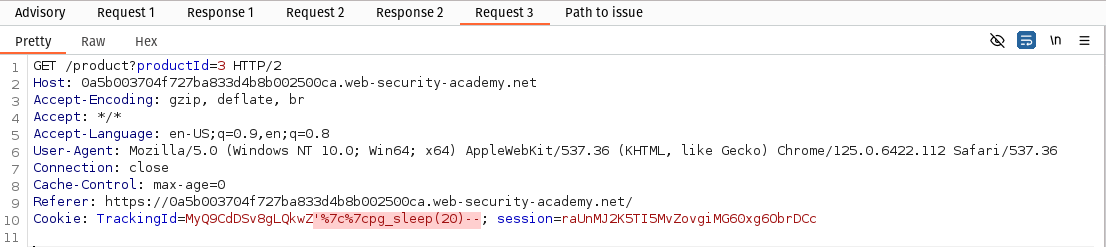
\includegraphics[width=1\textwidth]{slike/sql_requests.png}
  \caption{Zahtjev koji je otkrio bazu podataka i iskoristio SQL ranjivost}
  \label{slk:burp_auto}
\end{figure}

Pod karticom \textit{Advisory} s slike \ref{slk:burp_auto} je vidjljivo koji CWE se krije iza otkrivene ranjivosti te detalje o ispitanoj ranjivosti. Sada je potrebno iskoristiti ovo znanje prilikom napada web aplikacije te potom izvršiti prijavu kao \textit{administrator}.
Prvo se navigira u karticu \textit{Proxy > HTTP history}. Ondje se nalazi GET zahtjev za putanju \textit{/login} te je potrebno modificirati dio kolačića gdje piše \textit{TrackingId} tako da na kraj vrijednosti stoji '.
To će natjerati stranicu da izbaci pogrešku iz kojeg se otkriva cijeli SQL upit što je vidljivo na slici \ref{slk:err_test}.

\begin{figure}[]
    \begin{lstlisting}[frame=single, breaklines]
        Unterminated string literal started at position 52 in SQL SELECT * FROM tracking WHERE id = 'JhlbaDuQVof0JeOw''. Expected char
    \end{lstlisting}
    \caption{Dobivena pogreška}
    \label{slk:err_test}
\end{figure}

Sada je potrebno modificirati taj zahtjev kako bi došli do lozinke korisnika \textit{administrator}. Dobar bi pokušaj bio potpuno maknuti vrijednost \textit{TrackingId} argumenta i zamijeniti ju sa zloćudnim SQL upitom.
Koristeći Repeater modul (desni klik na zahtjev > \textit{Send to Repeater}) te ćemo ondje izmijeniti vrijednost tako da sad u payload-u piše: \newline
\textit{TrackingId=' AND 1=CAST((SELECT username FROM users LIMIT 1) AS int)--}

Iz prijašnje greške \ref{slk:err_test} može se zaključiti da aplikacija traži samo jedan \textit{TrackingId} te da je vjerojatno potrebno ograničiti upit na jedan redak baze kao i jedan stupac.
Sada bi trebala doći nova greška koja kaže kako \textit{administrator} nije tipa \textit{integer}. Iz ove greške je očito da se administrator nalazi prvi na popisu. Kao što je vidljivo potrebno je pretvoriti polja koja nisu \textit{integeri} u \textit{int} upravo kako bi 
natjerali bazu da "procuri informacije".
Ponovno ćemo se sada vratiti u \textit{Repeater} te ponoviti prijašnji zahtjev s malom preinakom:\newline
\textit{TrackingId=' AND 1=CAST((SELECT password FROM users LIMIT 1) AS int)--}

Ovaj upit napokon otkriva password za korisnika \textit{administrator} \ref{slk:err_good} no kao grešku.
\begin{figure}[H]
    \begin{lstlisting}[frame=single, breaklines]
        ERROR: invalid input syntax for type integer: "vuapcoxchp374pzq5d31"
    \end{lstlisting}
    \caption{Pogreška koja ispisuje lozinku za administratora}
    \label{slk:err_good}
\end{figure}
\newpage % dodano radi urednosti
\subsection{Vježba 1: ZAP}
Najprije u gornjem desnom kutu alat je potrebno postaviti \textit{Mode} na ATTACK. Zatim je potrebno kliknuti na \textit{Automated scan} i unijeti link mete.
Skeniranje traje nešto dulje od Burpovog. Među alertima je vidljivo da ZAP nije primijetio da uopće postoji mogućnost SQL injection-a\ref{slk:zap_vuln}. Prije je spomenuto kako ZAP ima Fuzzer ali nije trenutno funkcionalan. Razlog tomu je što ZAP trenutno nema mogućnost 
skeniranja HTTP zaglavlja što je veliki minus u odnosu na Burp.\cite{burp_to_zap} Ovaj zadatak služi otkrivanju ove velike manjkavosti ZAP-a nad Burpom.
\begin{figure}[H]
    \centering
    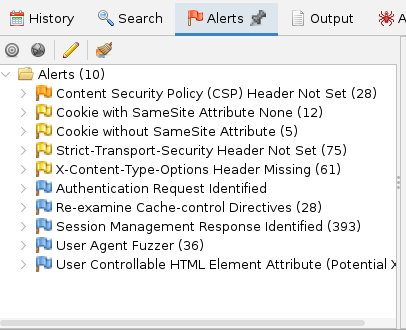
\includegraphics[width=0.8\textwidth]{slike/zap_sql_alerts.png}
    \caption{Manjak upozorenja na ranjivosti web aplikacije}
    \label{slk:zap_vuln}
\end{figure}

Problem je moguće zaobići koristeći ZAP HUD.\@ To je modul koji omogućava ručnu provjeru, izmjenu i slanje zahtjeva. Nakon što se uključi \textit{Break} prilikom gledanja \textit{/login} putanje nakon klika na gumb Login.
Ovdje je potrebno izmijeniti HTTP zaglavlje te modificirati kolačić kao što je prethodno to učinjeno za Burp. Naravno sada je otkriveno dobro rješenje na isti način kao i za Burp.
%%%%%%%%%%%%%%%%%%%%%%%%%%%%%%%%%%%%%%%%%%%%%%%%%%%%%%%%%%%%%%%%%%%%%%%%%%%%%%%%%%%%%%%%
%     2FA
%%%%%%%%%%%%%%%%%%%%%%%%%%%%%%%%%%%%%%%%%%%%%%%%%%%%%%%%%%%%%%%%%%%%%%%%%%%%%%%%%%%%%%%%
\newpage % dodano radi urednosti
\section{Dvofaktorska autentifikacija sa pogrešno konfiguriranom logikom}
%\subsection{Općenito}
Dvofaktorska autentifikacija (2FA) je sigurnosni mehanizam koji koristi dva različita faktora za provjeru identiteta korisnika, kao što 
su lozinka (prvi faktor) i jednokratni kod poslan putem SMS-a ili aplikacije (drugi faktor). Iako 2FA značajno povećava sigurnost, može 
biti ranjiv na određene vrste napada ako nije pravilno implementiran.\cite{dmitrienko2014security,aloul2009two}
Primjeri loše implementacije su recikliranje sigurnosnih kodova, realizacija 2FA na klijentskoj strani, direktan pristup API-ju, loša programska potpora i mnogi drugi.

Ova laboratorijska vježba ima ranjivost u dvofaktorskoj autentifikaciji zbog pogrešne logike, konkretno uz zahtjev za unos sigurnosnog koda u kolačiću prenosi i ime korisnika te nema limit na slanje zahtjeva što uvelike kompromitira aplikaciju.
Za rješavanje zadataka, potrebno je pristupiti računu korisnika \textit{Carlosa}.
Kao informacije za vježbu su pruženi podatci za pristup korisniku \textit{wiener} s lozinkom \textit{peter} te pristup mail serveru.\cite{2FA_lab}
Također je dan hint kako se korisnik \textit{carlos} neće pokušati ulogirati za vrijeme trajanja napada.

\subsection{Testiranje: Burp Suite}
Skeniranje se pokreće kao u prethodnoj vježbi. 
Kao u stvarnim situacijama, zanimljivi su POST zahtjevi koje skener šalje. 
Pokušat će se iskoristiti \textit{/login} putanja za rješavanje vježbe. 
Prije svega, pokušava se ulogirati s danim vjerodajnicama, nakon čega se traži unos 4-znamenkastog koda koji je poslan na mail. 
Već sada se uočava manjkavost realizacije. 
Ako kod ima samo 4 znamenke, to znači da postoji samo 10,000 mogućih kombinacija što nije puno za današnje sustave. 
Nakon što se uspije, pretražit će se povijest skeniranja da se vidi kako se zahtjev može izmijeniti.

Zahtjev sa putanjom \textit{/login2} šalje se na \textit{Intruder} kao što je vidljivo na slici \ref{slk:burp_req}. 
Jednom kada se uđe u Intruder, vrijednost \textit{verify} iz \textit{wiener} mijenja se u \textit{carlos} za GET zahtjev, što generira privremeni kod. 
Zatim se POST zahtjev iste putanje šalje na Intruder te se bira način rada \textit{Sniper} i označava vrijednost polja \textit{mfa-code} za modificirani payload što je vidljivo na \ref{slk:burp_req_config}. 
Burp će sada slati zahtjeve, svaki put modificirajući payload, kako bi pogodio točan kod za carlosa.

\begin{figure}[H]
  \centering
  \begin{minipage}[b]{0.45\textwidth}
    \centering
    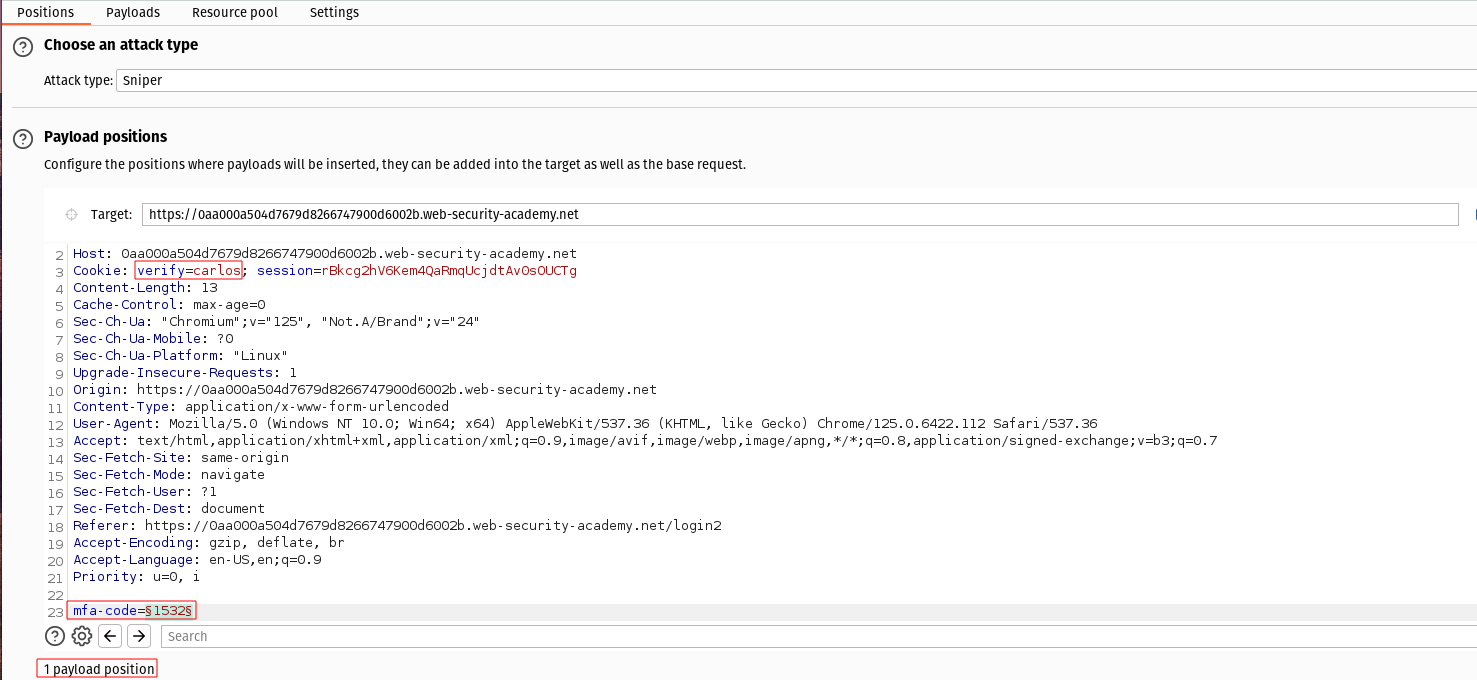
\includegraphics[width=\textwidth]{slike/intruder_2fa.png}
    \caption{Zahtjev koji ćemo koristiti u Intruderu}
    \label{slk:burp_req}
  \end{minipage}
  \hspace{0.05\textwidth} % Razmak između slika
  \begin{minipage}[b]{0.45\textwidth}
    \centering
    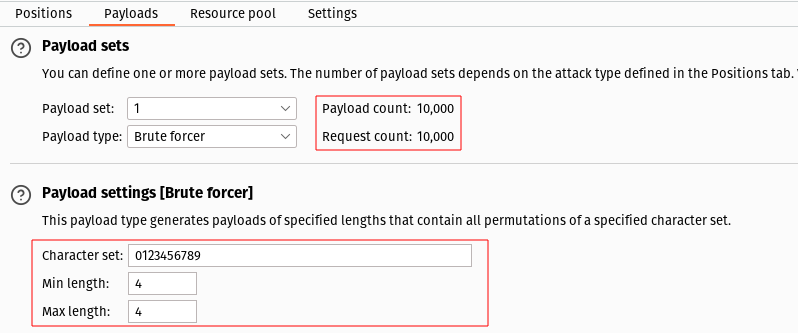
\includegraphics[width=\textwidth]{slike/payload_intruder.png}
    \caption{Konfiguriranje payloada}
  \end{minipage}
  \label{slk:burp_req_config}
\end{figure}

Sada se traži odgovor koji se razlikuje od drugih ili po duljini ili po vrsti odgovora. U ovom slučaju razlikovat će se i po vrsti i po duljini odgovora\ref{slk:burp_atks}. Jedan jedini payload vratio se s odgovorom 302, što označava redirekciju. Kada se pogleda vrijednost payloada za taj zahtjev, vidi se da je Carlosov trenutačni kod 0100.
\begin{figure}[H]
  \centering
  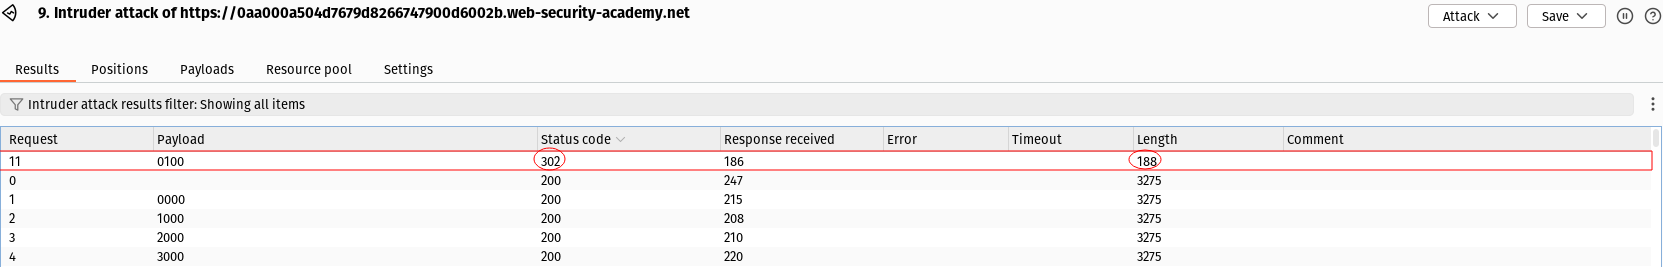
\includegraphics[width=1\textwidth]{slike/intruder_atk.png}
  \caption{Prikaz napada uz modul Intruder}
  \label{slk:burp_atks}
\end{figure}

Odgovor se učita u pretraživač ili se kod ručno unese, čime se završava vježba. Pritom se mora paziti da se na preostalim zahtjevima za vrijednost \textit{verify} upiše \textit{carlos}.\newpage % dodano radi urednosti

\subsection{Testiranje: ZAP}
Kako je već mnogo poznato o web aplikaciji, testiranje se može brže provesti. Sa ZAP HUD-om se ponovno normalno ulogira kao što je to učinjeno kod Burpa. Nakon što se ulogira s danim vjerodajnicama, otići će se u karticu \textit{History} u glavnom izborniku. Ondje se izabire GET zahtjev za \textit{/login2} putanju, te mu se modificira vrijednost \textit{verify} i zahtjev se šalje.

Zatim se pronađe stari POST zahtjev za \textit{/login2}. Kako generator regularnih izraza nije funkcionalan u ZAP-u, potrebno je napraviti kratki "obilazak". Prvo se dodaje generator zahtjeva tipa \textit{Numberzz}, koji stvara brojeve od 0 do 9999 što je vidljivo na slici \ref{slk:zap_gen}. Nakon toga je iz slike \ref{slk:zap_config_proc} vidljivo da je potrebno namjestiti procesor za zahtjeve koji će zahtjeve pretvoriti u oblik koji je zapravo potreban.
\begin{figure}[H]
  \centering
  \begin{minipage}[b]{0.5\textwidth}
    \centering
    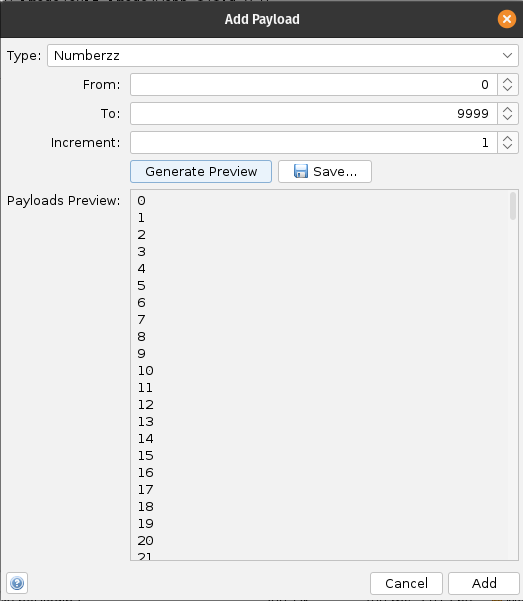
\includegraphics[width=\textwidth]{slike/payload_fuzz.png}
    \caption{Dodavanje generatora}
    \label{slk:zap_gen}
  \end{minipage}
  \hspace{0.05\textwidth} % Razmak između slika
  \begin{minipage}[b]{0.4\textwidth}
    \centering
    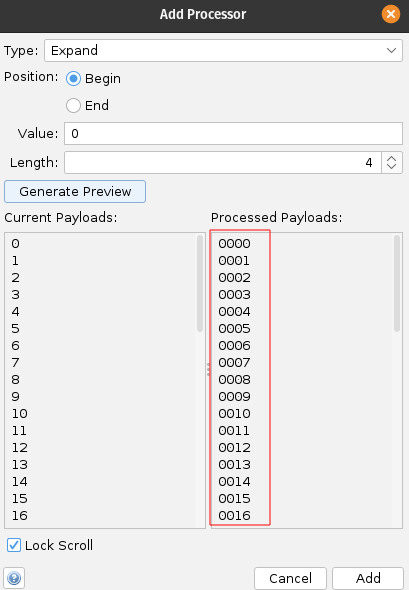
\includegraphics[width=\textwidth]{slike/processor_fuzz.png}
    \caption{Konfiguriranje procesora zahtjeva}
    \label{slk:zap_config_proc}
  \end{minipage}
\end{figure}

Kao i u radu s Burpom sada se pronalazi odgovor koji se razlikuje te se šalje pregledniku. Nakon toga bi se trebalo pojaviti na zaslonu nešto kao na slici \ref{slk:zap_succ}.

\begin{figure}[H]
  \centering
  
\includegraphics[width=0.4\textwidth]{slike/2fa_succ.png}
  \caption{Prikaz uspješne prijave}
  \label{slk:zap_succ}
\end{figure}
%%%%%%%%%%%%%%%%%%%%%%%%%%%%%%%%%%%%%%%%%%%%%%%%%%%%%%%%%%%%%%%%%%%%%%%%%%%%%%%%%%%%%%%%
%     Brute force
%%%%%%%%%%%%%%%%%%%%%%%%%%%%%%%%%%%%%%%%%%%%%%%%%%%%%%%%%%%%%%%%%%%%%%%%%%%%%%%%%%%%%%%%
\section{Napad silom na lozinku koristeći lošu implementaciju promjene lozinke}
Napad grubom silom na lozinku podrazumijeva isprobavanje svih mogućih kombinacija dok se ne pronađe točna. 
Kada se kombinira s loše implementiranom funkcionalnošću promjene lozinke, mogu se pojaviti ozbiljni sigurnosni problemi. 
Primjerice, ako sustav dopušta korisniku da promijeni lozinku bez provjere identiteta putem adekvatnih metoda (npr. slanje privremene lozinke na unaprijed spremljeni mail, korištenje dvofaktorske autentifikacije), otvara se prostor za iskorištavanje ranjivosti.
U takvim scenarijima, napadač koji dobije pristup korisničkom računu putem metoda poput napada grubom silom ili socijalnog inženjeringa može lako promijeniti lozinku i time zaključati legitimnog korisnika. 
To se događa jer sustav ne provjerava dovoljno identitet korisnika prije nego što dopusti promjenu lozinke.

Kako bi se smanjili rizici, ključno je implementirati robustne sigurnosne mjere poput dvofaktorske autentifikacije, obavijesti o promjeni lozinke na registrirani virtualni sandučić (engl. \textit{mail}), specifične fraze koje se generiraju za svakog korisnika pri registraciji i slična rješenja.
Nažalost, napade grubom silom je gotovo nemoguće spriječiti te bi dizajneri trebali ciljati na to da je ovo najbolji mogući napad koji se pruža napadačima jer je ekstenzivan te u puno slučajeva zahtjeva puno vremena i resursa.\cite{knudsen2011brute} 

Sigurnosni propust u funkcionalnosti promjene lozinke u ovoj laboratorijskoj vježbi čini ju podložnom napadima grubom silom. Za rješavanje ove vježbe, potrebno je iskoristiti listu potencijalnih lozinki kako bi se pristupilo Carlosovom korisničkom računu. 
Informacije koje su na raspolaganju uključuju vlastite vjerodajnice (wiener:peter), korisničko ime \textit{carlos}, te listu kandidata za lozinku u obliku teksta gdje je svaka potencijalna lozinka zapisana u zaseban redak.\cite{brute_lab}
\newpage %dodano radi preglednosti
\subsection{Testiranje: ZAP}
Prije nego što se započne s ručnim testiranjem aplikacije, provest će se automatizirani sken kako bi se dobila mapa povezanih stranica (engl. \textit{sitemap}). 
Iako neće puno pomoći u rješavanju ove konkretne vježbe, uvijek je dobra praksa ispitati površinu napada kako bi se mogao pronaći dobar vektor napada. 
Sken sam po sebi ne otkriva previše, tako da će se pristupiti ručnom testiranju aplikacije uz pomoć ZAP HUD-a.

Prva stvar koja će se napraviti je prijava s danim vjerodajnicama kako bi se vidjelo kako aplikacija gradi zahtjeve za prijavu. 
Za to će poslužiti modul \textit{Break}, koji omogućuje pregled i uređivanje svakog zahtjeva prije nego što ga preglednik pošalje i odgovora prije nego što ga preglednik primi. 
Iako naslov vježbe sugerira da vjerojatno neće biti moguće iskoristiti funkcionalnost prijave, dobro je biti temeljit i vidjeti postoji li neka ranjivost koja nije namjerno ostavljena. 
U ovom konkretnom slučaju, prijava je dobro implementirana, te će se nastaviti s testiranjem. 
Sada je zaslon nakon prijave nešto drukčiji nego na prijašnjim vježbama kao što je vidljivo na slici \ref{slk:succ_login}. Vidljivo je da je osim unosa maila moguća i promjena lozinke ukoliko je poznata trenutna.
\begin{figure}[H]
  \centering
  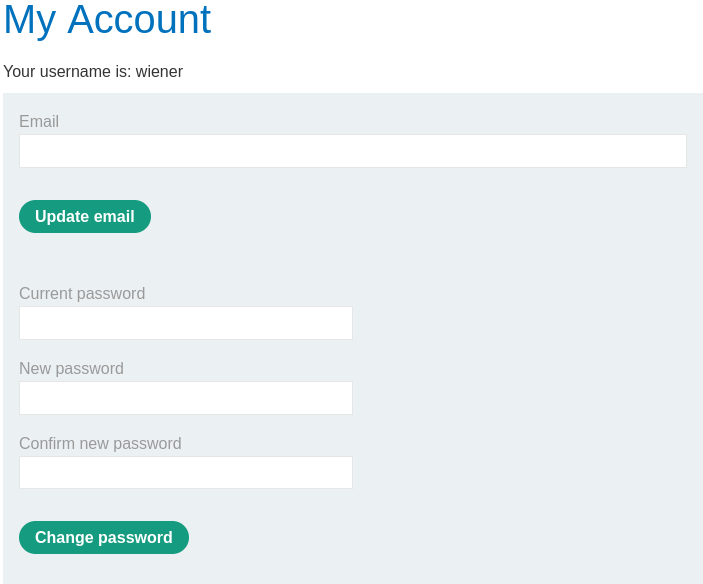
\includegraphics[width=0.6\textwidth]{slike/b_f_postLogin.png}
  \caption{Sučelje nakon prijave sa dostupnim vjerodajnicama}
  \label{slk:succ_login}
\end{figure}

Očito je da se mora dokučiti kako iskoristiti opcije za mijenjanje lozinke. 
Pokušat će se promijeniti lozinka računu kojem se ima pristup kako bi se vidjelo kako web aplikacija gradi zahtjev. 
Ponovno će se koristiti \textit{Break} funkcionalnost kako bi se presreo i uredio zahtjev vidljiv na slici \ref{slk:gen_req}. 
Označeno je tijelo zahtjeva koje je potrebno urediti.

\begin{figure}[H]
  \centering
  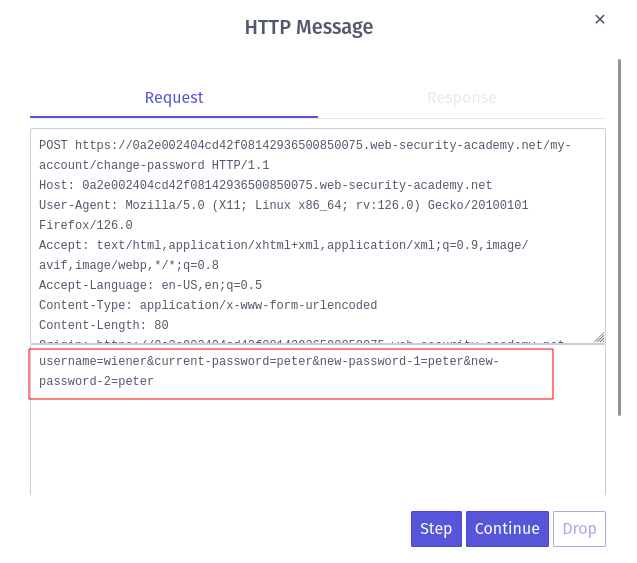
\includegraphics[width=0.8\textwidth]{slike/break_np.png}
  \caption{Zahtjev koji aplikacija generira}
  \label{slk:gen_req}
\end{figure}

Iz slike \ref{slk:gen_req} je vidljivo da se, kao u prijašnjim vježbama, može mijenjati korisničko ime kao i pripadajuća lozinka. 
Sada, kada su te putanje spremljene, koristit će se \textit{Fuzzer} kako bi se razotkrila lozinka za korisnika \textit{carlos}. 
Kako izmjena lozinki zapravo nije moguća, potrebno je na drugi način dokučiti koja je lozinka točna.
Relevantni POST zahtjev šalje se u \textit{Fuzzer}. 
Unutar \textit{Fuzzer}a korisničko ime \textit{wiener} zamjenjuje se s \textit{carlos}, a trenutna lozinka označava se kao mjesto na kojem će alat pogađati lozinke. 
Također, alat se opskrbljuje kandidatima za lozinku koji su dobiveni na početku vježbe, te se postavljaju različite nove lozinke. 
To se radi kako bi se umjesto pogreške da je lozinka netočna dobio odgovor koji javlja da se nove lozinke ne poklapaju. 
Primjer tako definiranog zahtjeva možemo vidjeti na slici \ref{slk:full_config_fuzz_zap}

\begin{figure}[H]
  \centering
  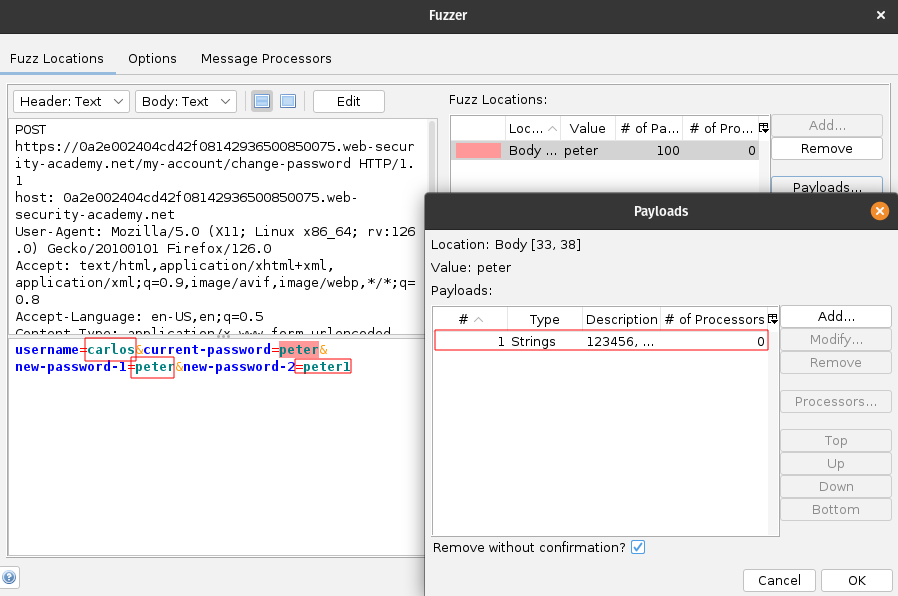
\includegraphics[width=1\textwidth]{slike/zap_fuzz_pass.png}
  \caption{Ispravno konfiguriran \textit{Fuzzer}}
  \label{slk:full_config_fuzz_zap}
\end{figure}

Sada se traži odgovor koji, među onima kojima su zaprimljeni ima različitu duljinu odgovora. 
Uz njega nam piše i koju je lozinku alat pokušao poslati. 
Sada je potrebno tu lozinku iskoristiti da za prijavu kao \textit{carlos} i tako završava ova laboratorijska vježba.

\newpage %dodano radi preglednosti
\subsection{Testiranje: Burp Suite}
Kao i za ZAP, aplikacija će se prvo skenirati kako bi se utvrdila površina napada. 
Kao i kod ZAP-a, skener nije utvrdio nikakve probleme. 
Unese se ispravna trenutna lozinka i dvije nove lozinke koje se ne podudaraju. 
Ovaj zahtjev POST /my-account/change-password šalje se u Burp Intruderu. 
Zbog prijašnjeg testiranja, zna se da je potrebno pratiti razlike u odgovorima.
U Burp Intruderu parametar username mijenja se u carlos i dodaje se položaj za promjenu za parametar trenutne lozinke. 
Provjerava se da su parametri za nove lozinke postavljeni na dvije različite vrijednosti. 
Na kartici \textit{Payloads} unosi se lista lozinki.
Kada je napad završen, može se primijetiti da je jedan odgovor drukčije duljine i sadrži poruku "Nove lozinke se ne podudaraju". 
Lozinka koja je iskorištena u tom zahtjevu je lozinka za račun \textit{carlos} što je vidljivo na slici \ref{slk:atk_end}.

\begin{figure}[H]
  \centering
  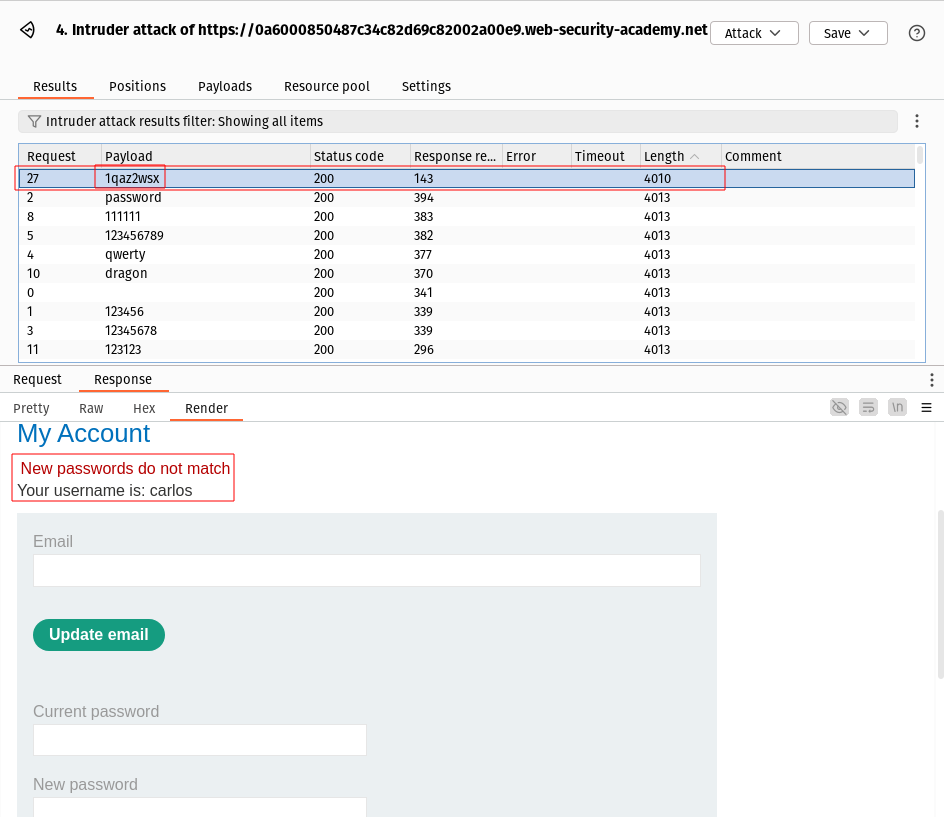
\includegraphics[width=1\textwidth]{slike/butp_bf_fuzz.png}
  \caption{Kraj napada u \textit{Intruder}u}
  \label{slk:atk_end}
\end{figure}
Rješenje u ovom slučaju je \textbf{1qaz2wsx} što je i vidljivo iz slike \ref{slk:atk_end}.